\documentclass[runningheads]{llncs}
\usepackage{graphicx}
\usepackage[T1]{fontenc}
\usepackage[utf8]{inputenc}
\usepackage{xcolor}
\usepackage{listings}
\definecolor{vsblue}{RGB}{0, 0, 255}
\definecolor{vsdarkgreen}{RGB}{0, 128, 0}
\definecolor{vsorange}{RGB}{255, 165, 0}
\definecolor{vsgray}{RGB}{128, 128, 128}
\definecolor{vscomment}{RGB}{0, 128, 0}
\lstset{
    basicstyle=\ttfamily,
    breaklines=true,
    postbreak=\mbox{\textcolor{red}{$\hookrightarrow$}\space},
    keywordstyle=\color{vsblue},
    stringstyle=\color{vsorange},
    commentstyle=\color{vscomment},
    numbers=left,
    numberstyle=\tiny\color{vsgray},
    stepnumber=1,
    numbersep=5pt,
}
\begin{document}
\title{OnlineInfoOlympiad}
\author{Ghionea Petru-Daniel}
\institute{Universitatea "Alexandru Ioan Cuza" din Iasi}
\maketitle
\begin{abstract}
OnlineInfoOlympiad este o aplicație ce simulează o olimpiadă online de informatică, permitând conectarea mai multor utilizatori folosind un model client-server. Aplicația analizează soluțiile primite de la utilizatori și transmite înapoi nota obținută.
\end{abstract}
\keywords{Olimpiada online, Model client-server, Corectare automată}
\section{Introducere}
Scopul acestui proiect este crearea unui model client-server interactiv și ușor de utilizat pentru o olimpiadă online de informatică. Obiectivele acestui proiect sunt:
\begin{itemize}
  \item Automatizarea: Dezvoltarea unui sistem de evaluare automată a soluțiilor trimise de utilizatori.
  \item Feedback-ul: Oferirea unui feedback utilizatorilor cu privire la corectitudinea soluțiilor acestora și punctajului obținut.
  \item Extensibilitatea: Crearea unei arhitecturi ce permite adăugarea de noi funcționalități și îmbunătățiri ulterioare.
\end{itemize}
\section{Tehnologii aplicate}
Această aplicație folosește modelul TCP/IP (Transmission Control Protocol/Internet Protocol) utilizat pentru a permite comunicarea între dispozitivele dintr-o rețea. Format din patru nivele și anume:
\begin{enumerate}
  \item Nivelul fizic: Asigură conectarea host-ului la rețea.
  \item Nivelul rețea: Permite gazdelor să emită pachete în orice rețea; pachete care vor circula independent până la destinație.
  \item Nivelul transport: Asigură realizarea comunicării între gazda sursă și gazda destinație.
  \item Nivelul aplicație: Conține protocoale de nivel înalt și este cel mai apropiat de utilizator, oferind o interfață pentru aplicația care utilizează rețeaua.
\end{enumerate}
\hspace{1em} La nivelul transport, dintre protocolul TCP și protocolul UDP, chiar dacă protocolul UDP este mai rapid, acesta nu oferă garanții privind livrarea sau ordinea datelor, nu are control de flux, deci nu așteaptă o confirmare de primire de la destinatar înainte de a transmite următorul pachet și nu este un protocol orientat-conexiune, deci nu stabilește o conexiune înainte de a trimite date.

Toate aceste aspecte sunt necesare pentru a simula un concurs de tip olimpiadă, deci a fost ales protocolul TCP.
\section{Structura aplicației}
Pentru modelarea acestei aplicații au fost folosite următoarele concepte:
\begin{itemize}
    \item Sockets: Sunt utilizate funcțiile din \texttt{<sys/socket.h>} pentru a crea și gestiona socket-uri ce permit comunicarea între server și client.
    \item Forking: Este utilizată funcția \texttt{fork()} în server pentru a crea procese fiu ce vor comunica cu un client în parte, permitând astfel acceptarea simultană a mai multor clienți.
    \item Manipularea de fișiere: Serverul citește conținutul fișierului de configurare și al problemei alese folosind funcții precum \texttt{fopen} sau \texttt{fread}.
    \item Manipularea de directoare: Este utilizată o funcție custom pentru a determina calea completă a unui fișier până la un anumit director.
    \item Generare aleatoare: Serverul alege în mod aleatoriu problema ce urmează a fi rezolvată de către client, utilizând funcția \texttt{rand()} pentru a genera un număr aleatoriu.
    \item Aplicarea conceptelor de concurență: serverul folosește primitiva \texttt{select()} pentru a gestiona conectarea clienților la server într-un anumit timp.
    \item Gestionarea timpului: sunt utilizate primitivele \texttt{time()} și \texttt{clock()} pentru a monitoriza timpul de rezolvare al clientului.
    \item Memorie partajată: serverul folosește un flag partajat în memorie pentru a trimite problema ce trebuie rezolvată clienților în același timp.
    \item Compilare și execuție: serverul compilează și rulează soluția clientului folosind apeluri de sistem.
    \item Validarea rezultatelor: serverul compară rezultatul obținut de la client cu soluția corectă și acordă o notă în funcție de timpul de executie, corectitudinea soluției și timpul de upload.
\end{itemize}
\hspace{1em} De asemenea, a fost creată o diagramă pentru a conceptualiza mai ușor aplicația(vezi figura 1).
\begin{figure}[h]
    \centering
    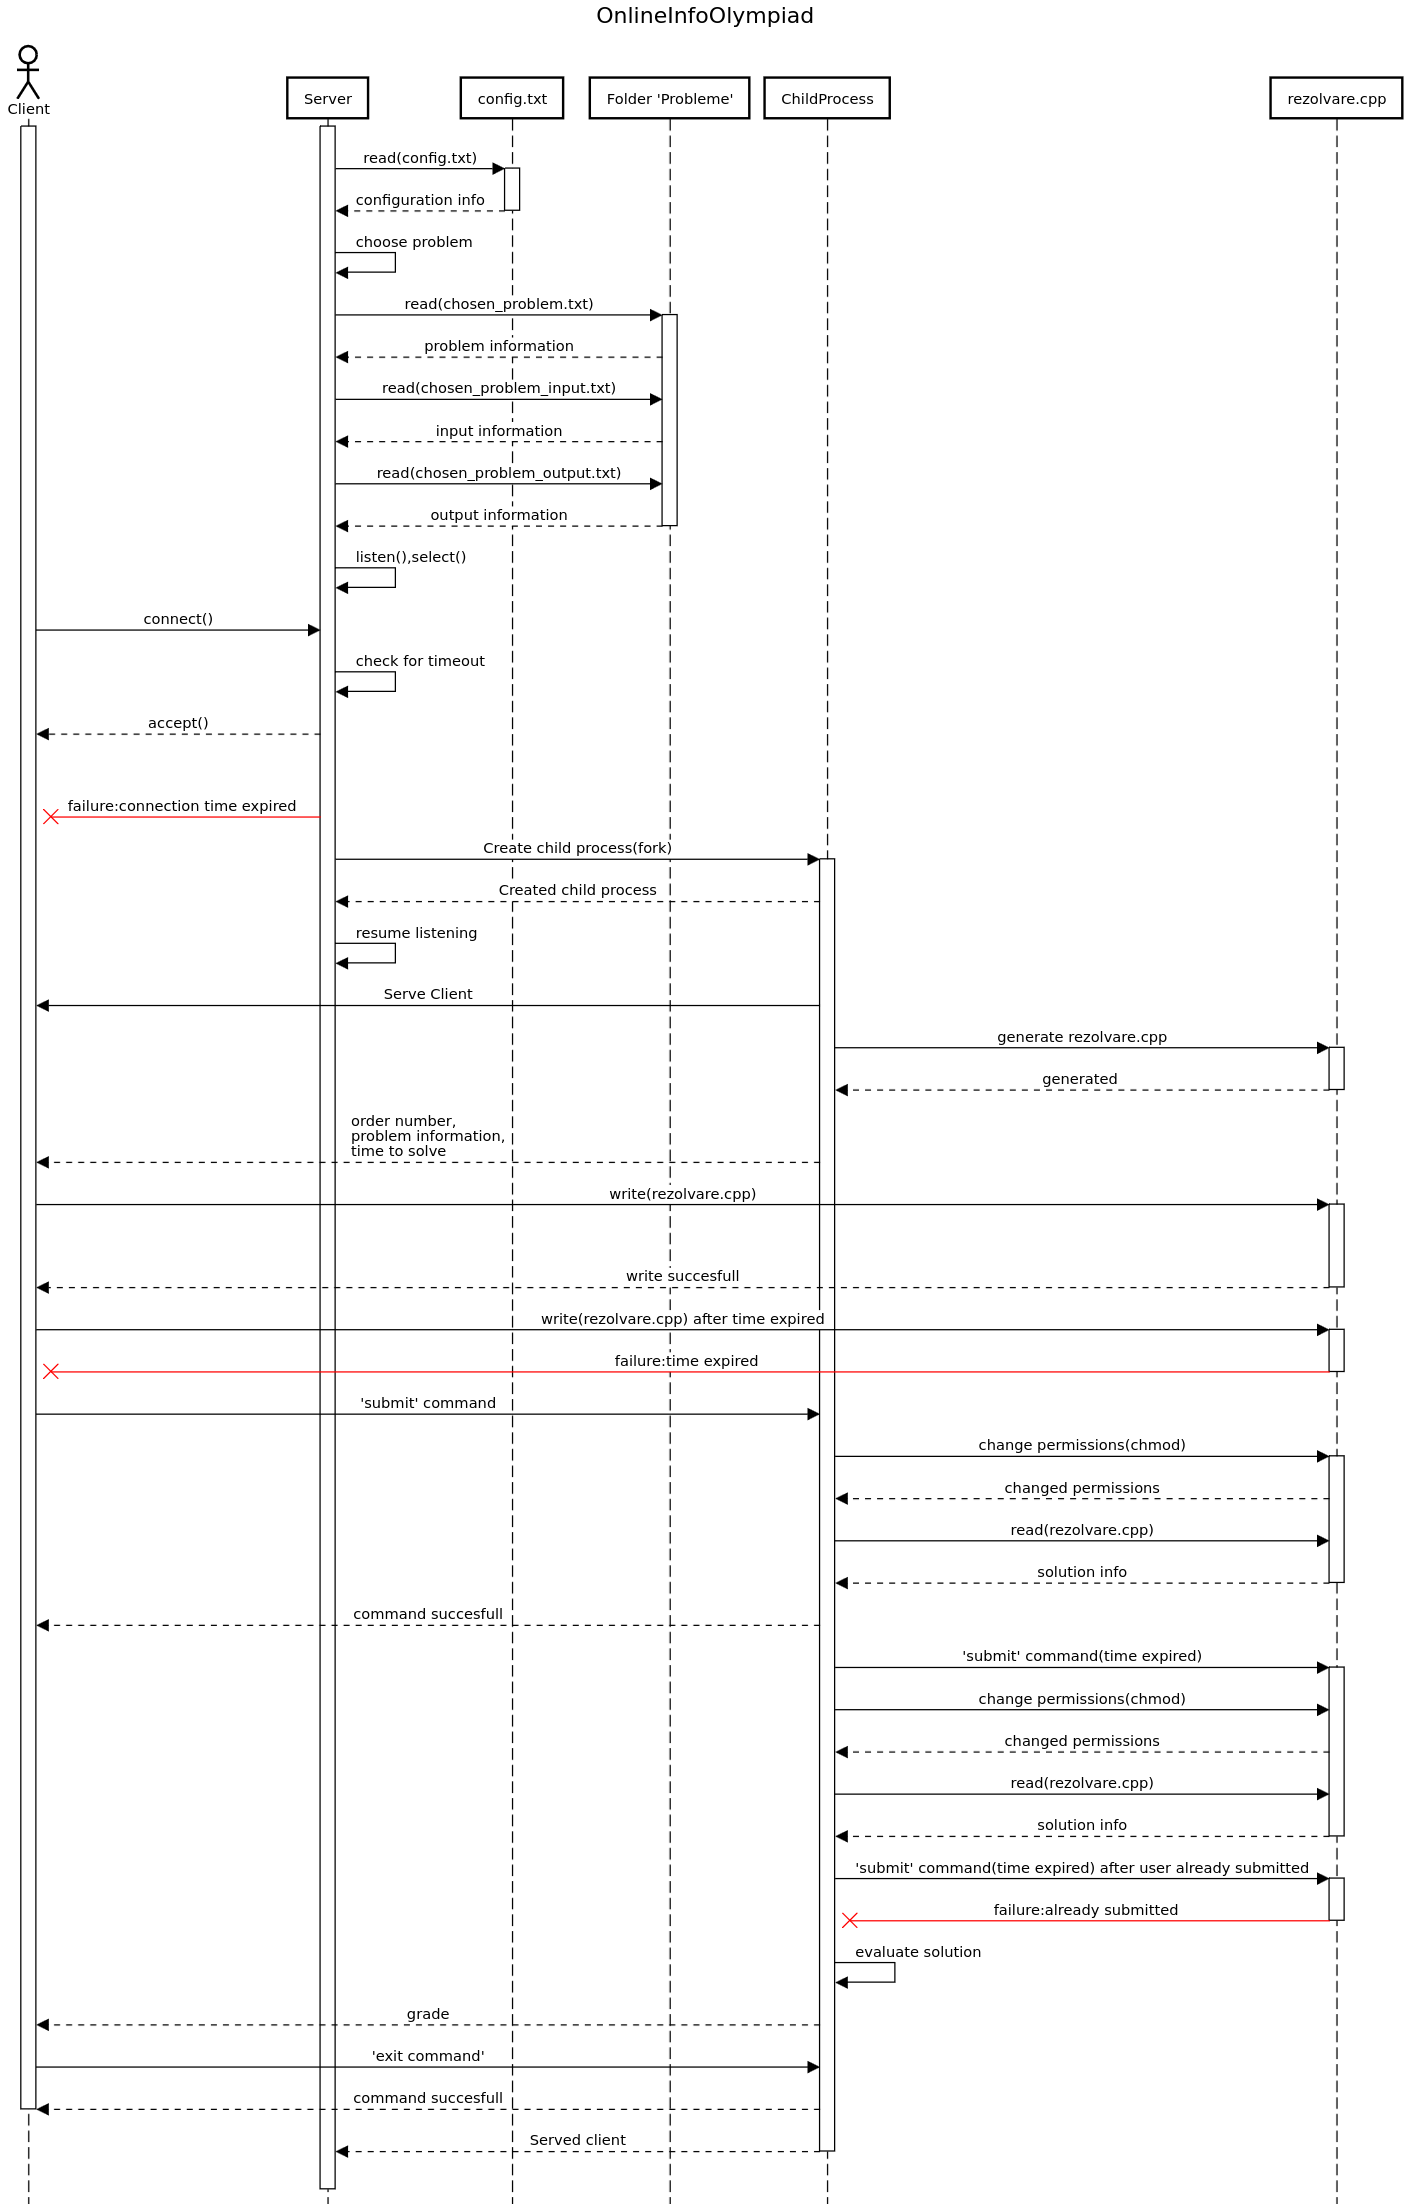
\includegraphics[width=0.7\textwidth]{OnlineInfoOlympiad.png}
    \caption{Diagrama aplicatiei}
    \label{fig:OnlineInfoOlympiad}
  \end{figure}
\section{Aspecte de implementare}
Aplicația va urma următorul protocol de comunicare:
\begin{itemize}
    \item Conectarea: Serverul așteaptă conexiuni la portul 2000 folosind primitiva \texttt{listen}; iar clientul se conectează la adresa serverului și portul specificate în linia de comandă folosind primitiva \texttt{connect}.De asemenea, este utilizată primitiva \texttt{'select'} pentru a aloca un anumit timp de conectare. Dacă acest timp expiră, problema ce trebuie rezolvată va fi trimisă clienților și nu vor mai fi acceptate conexiuni.
    \item Inițierea comunicării: După conectare, serverul trimite problema selectată clientului împreună cu timpul alocat rezolvării și va genera fișierul în care se va scrie rezolvarea.
    \item Comunicarea propriu-zisă: Clientul va transmite serverului comenzi și va citi răspunsurile primite folosind primitivele \texttt{read} și \texttt{write}. Serverul va utiliza aceleași primitive pentru a citi comenzile și a transmite răspunsurile. De asemenea, clientul va avea lista de comenzi disponibile și va aștepta introducerea unei comenzi de către utilizator.
    \item Gestionarea timpului alocat rezolvării: După expirarea timpului alocat, serverul va schimba permisiunile de acces la fișierul în care se află rezolvarea, va copia rezolvarea clientului, o va compila și corecta. De asemenea, corectarea va începe și dacă utilizatorul introduce comanda 'submit'.Corectarea constă în compararea fișierului de output al clientului cu fișierul de output corect. Se va asigna o notă în funcție dacă fișierul de output este corect, parțial corect sau incorect; precum și în funcție de timpul de execuție și timpul de upload.
    \item Încheierea conexiunii: Dacă utilizatorul introduce comanda 'exit', serverul va opri conexiunea cu acel client.
\end{itemize}

\hspace{1em}Într-un scenariu real, aplicația ar putea fi utilizată în următorul mod:

\hspace{1em}Un profesor coordonator ce va rula aplicația server va modifica fișierul de configurare stabilind numărul maxim de clienți, timpul alocat pentru rezolvarea problemei alese și timpul alocat conectării..
Elevii ce participă la concurs vor rula pe mașinile proprii aplicația client specificând în linia de comandă adresa IP și portul, atât timp cât nu depășesc timpul alocat conectării..
Aplicația server va alege în mod aleator o problemă și va trimite clientilor informații despre aceasta, precum și timpul alocat rezolvării.

\hspace{1em}Elevii vor rezolva problema în timpul alocat și vor scrie rezolvarea în fișierul denumit 'rezolvare.cpp' creat de server.
După terminarea rezolvării, elevii vor introduce comanda 'submit' pentru a notifica serverul să înceapă corectarea. După introducerea comenzii 'submit', elevul respectiv nu va mai avea acces la fișierul 'rezolvare.cpp' pentru a face modificări. De asemenea, după expirarea timpului alocat, comanda 'submit' va fi apelată în mod automat.
Serverul va corecta soluțiile și va nota fiecare elev în parte.
După primirea rezultatului obținut, elevul introduce comanda 'exit' pentru a se deconecta.

\hspace{1em} Secțiuni de cod importante:
\begin{lstlisting}[language=C, caption={Functia pentru obtinerea caii complete a unui fisier pana la un director specificat}, label={lst:getFullPathUntilDir}]
char* getFullPathUntilDir(const char* filePath, const char* targetDir)
{
  char currentDir[MAX_PATH_LENGTH];
  char fileName[MAX_PATH_LENGTH];
  char fileDir[MAX_PATH_LENGTH];
  
  // Obtine directorul de lucru curent
  if (getcwd(currentDir, MAX_PATH_LENGTH) == NULL)
  {
    perror("[server]Eroare la gasirea directorului curent de lucru.\n");
    return NULL;
  }
  
  // Creeaza calea completa a fisierului
  snprintf(fileName, MAX_PATH_LENGTH, "%s/%s", currentDir, filePath);
  
  // Copiaza calea completa intr-o alta variabila
  strncpy(fileDir, fileName, MAX_PATH_LENGTH);
  
  // Extrage directorul parinte al fisierului
  char* parentDir = dirname(fileDir);
  
  // Cauta directorul target in interiorul directorului parinte
  char* targetDirPos = strstr(parentDir, targetDir);
  
  // Verifica daca directorul target a fost gasit
  if (targetDirPos != NULL)
  {
    // Calculeaza lungimea subsirului de la inceputul directorului parinte pana la sfarsitul directorului target
    size_t length = targetDirPos - parentDir + strlen(targetDir);
  
    // Aloca memorie pentru subsir
    char* fullPath = malloc(length + 1);
  
    // Verifica daca alocarea de memorie a reusit
    if (fullPath == NULL)
    {
      perror("[server]Eroare la malloc.\n");
      return NULL;
    }
  
    // Copiaza subsirul in memoria nou alocata
    strncpy(fullPath, fileName, length);
  
    // Adauga terminatorul de sir '\0'
    fullPath[length] = '\0';
  
    // Returneaza sirul alocat dinamic continand calea pana la directorul target
    return fullPath;
  }
  else
  {
    // Afiseaza un mesaj de eroare daca directorul target nu a fost gasit
    printf("[server]Eroare: Directorul target %s nu a fost gasit.\n", targetDir);
    return NULL;
  }
}
\end{lstlisting}
\begin{lstlisting}[language=C, caption={Functia `submit`}, label=submit-function]
int submit(int submit_time)
{
  ssize_t bytes_read;
  char buffer[MAX_CONTENT], solution[100];
  const char *filePath = "Proiect/Server/server.c";
  const char *targetDir = "Proiect";
  const clientDir[100];
  int nota;
    
  // Construieste calea catre fisierul solutiei clientului
  sprintf(clientDir, "/Client%d", contorclienti);
  char *fullPath = getFullPathUntilDir(filePath, targetDir);
  strcat(fullPath, clientDir);
  strcat(fullPath, "/rezolvare.cpp");
    
  // Creeaza un fisier pentru solutia clientului
  sprintf(solution, "solutie_client%d.cpp", contorclienti);
  int fd_destination = open(solution, O_CREAT | O_RDWR, 0777);
  int fd_source = open(fullPath, O_RDONLY);
    
  // Copiaza continutul solutiei clientului intr-un fisier nou
  while ((bytes_read = read(fd_source, buffer, MAX_CONTENT)) > 0)
  {
    write(fd_destination, buffer, bytes_read);
  }
    
  // Inchide descriptorii de fisiere
  close(fd_source);
  close(fd_destination);
    
  // Efectueaza evaluarea solutiei trimise
  nota = corectare(submit_time);
    
  // Returneaza rezultatul evaluarii
  return nota;
}
\end{lstlisting}
\begin{lstlisting}[language=C, caption={Functia `corectare`}, label=corectare-function]
int corectare(int submit_time)
{
  FILE *fd_out_corect, *fd_out_client;
  clock_t start_execution, end_execution;
  double execution_time, one_fourth, two_fourths, three_fourths, four_fourths;
  char solution[100], compiled[100], compilation_command[100], execution_command[100], nume_out[100];
  char buffer1[100], buffer2[100];
  int nota, ok = 1, partial_ok = 0;
      
  // Construieste numele fisierelor si comenzilor pentru compilare si executie
  sprintf(solution, "solutie_client%d.cpp", contorclienti);
  sprintf(compiled, "solutie_client%d", contorclienti);
  sprintf(compilation_command, "g++ -Wall %s -o %s", solution, compiled);
  sprintf(execution_command, "./%s", compiled);
      
  // Calculeaza intervalele de timp pentru evaluare
  one_fourth = secunde_rezolvare / 4;
  two_fourths = 2 * secunde_rezolvare / 4;
  three_fourths = 3 * secunde_rezolvare / 4;
  four_fourths = 4 * secunde_rezolvare;
      
  // Compileaza solutia clientului
  int compilation_result = system(compilation_command);
      
  if (compilation_result == 0)
  {
    start_execution = clock();
      
    // Executa solutia clientului
    int execution_result = system(execution_command);
      
    end_execution = clock();
    execution_time = (((double)(end_execution - start_execution)) / CLOCKS_PER_SEC) * 10000.0;
      
    if (execution_result == 0)
    {
      // Deschide fisierul de output corect si fisierul de output de la client
      fd_out_corect = fopen("correct_output.out", "r");
      switch (randomP)
      {
      case 1:
        sprintf(nume_out, "recyclebin%d.out", contorclienti);
        fd_out_client = fopen(nume_out, "r");
        break;
      case 2:
        sprintf(nume_out, "rufe%d.out", contorclienti);
        fd_out_client = fopen(nume_out, "r");
        break;
      case 3:
        sprintf(nume_out, "tairos%d.out", contorclienti);
        fd_out_client = fopen(nume_out, "r");
        break;
      }
      
      while (fgets(buffer1, sizeof(buffer1), fd_out_corect) != NULL && fgets(buffer2, sizeof(buffer2), fd_out_client) != NULL)
      {
        // Compara liniile din fisierele de output
        if (strcmp(buffer1, buffer2) == 0)
        {
          partial_ok = 1;
        }
        else if (strcmp(buffer1, buffer2) != 0)
        {
          ok = 0;
          break;
        }
      }
      
      // Asigneaza nota in functie de rezultatul compararii
      if (ok == 1)
      {
        if (execution_time <= 0.5 && submit_time <= one_fourth)
          nota = 10;
        else if (execution_time <= 1.0 && (submit_time <= one_fourth || submit_time <= two_fourths))
          nota = 9;
        else if (execution_time <= 2.0 && (submit_time <= one_fourth || submit_time <= two_fourths || submit_time <= three_fourths))
          nota = 8;
        else if (execution_time <= 3.0 && (submit_time <= one_fourth || submit_time <= two_fourths || submit_time <= three_fourths || submit_time <= four_fourths))
          nota = 7;
        else
          nota = 6;
      }
      else if (partial_ok == 1)
      {
        nota = 5;
      }
      else
      {
        nota = 4;
      }
    }
    else
    {
      // Afiseaza mesaj de eroare daca executia a esuat
      char run_error[100];
      sprintf(run_error, "[server]Eroare la executia clientului %d\n", contorclienti);
      perror(run_error);
    }
  }
  else
  {
    // Solutia nu a putut fi compilata
    nota = 3;
  }
      
  // Inchide dexcriptorii de fisiere si sterge fisierele create temporar
  fclose(fd_out_corect);
  fclose(fd_out_client);
  remove(solution);
  remove(compiled);
  remove(nume_out);
      
  // Returneaza nota
  return nota;
}
\end{lstlisting}
\section{Concluzii}
Soluția propusă ar putea fi îmbunătățită astfel:
\begin{itemize}
    \item Adăugarea unui clasament al elevilor în funcție de nota obținută.
\end{itemize}
\section{Referințe bibliografice}
\begin{enumerate}
    \item Site-ul cursului de rețele de calculatoare: \url{https://profs.info.uaic.ro/~computernetworks/cursullaboratorul.php}
    \item Site-ul profesorului de laborator: \url{https://www.andreis.ro/teaching/computer-networks}
    \item Site-ul folosit pentru a crea diagrama: \url{https://sequencediagram.org/}
\end{enumerate}
\end{document}
